%El principal objetivo del presente Trabajo Integrador es el de proveer una comunicación USB para desarrollos basados en FPGA. Por esto mismo, es fundamental sintetizar un circuito en el FPGA que sirva de nexo entre el desarrollo y la placa de interfaz.\\

%Es por esto que se utilizó 
Para la implementación de la comunicación de un desarrollo científico determinado, se requiere un nexo entre la síntesis del circuito y la memoria del controlador USB. Este vínculo se lleva a cabo mediante una pequeña MEA que ejecuta las señales de lectura y escritura. Esta MEA se desarrolla en lenguaje VHDL.\\

Se utiliza por esto la placa MOJO v3 desarrollada por la empresa Embedded Micro. Esta placa, la cual se observa en la Figura \ref{mojo}, posee un Spartan-VI de Xilinx. El FPGA brinda posibilidad de elaborar sistemas complejos de muy alta velocidad y permite al desarrollador de sensores y sistemas de adquisición de datos científicos la síntesis de circuitos que resuelvan problemas a la medida de los requerimientos. Dispone también de 84 puertos digitales configurables como entrada y/o salida, 8 entradas analógicas, 8 LED's de propósito general, un botón de tipo pulsador.\\

\begin{figure}
	\centering
	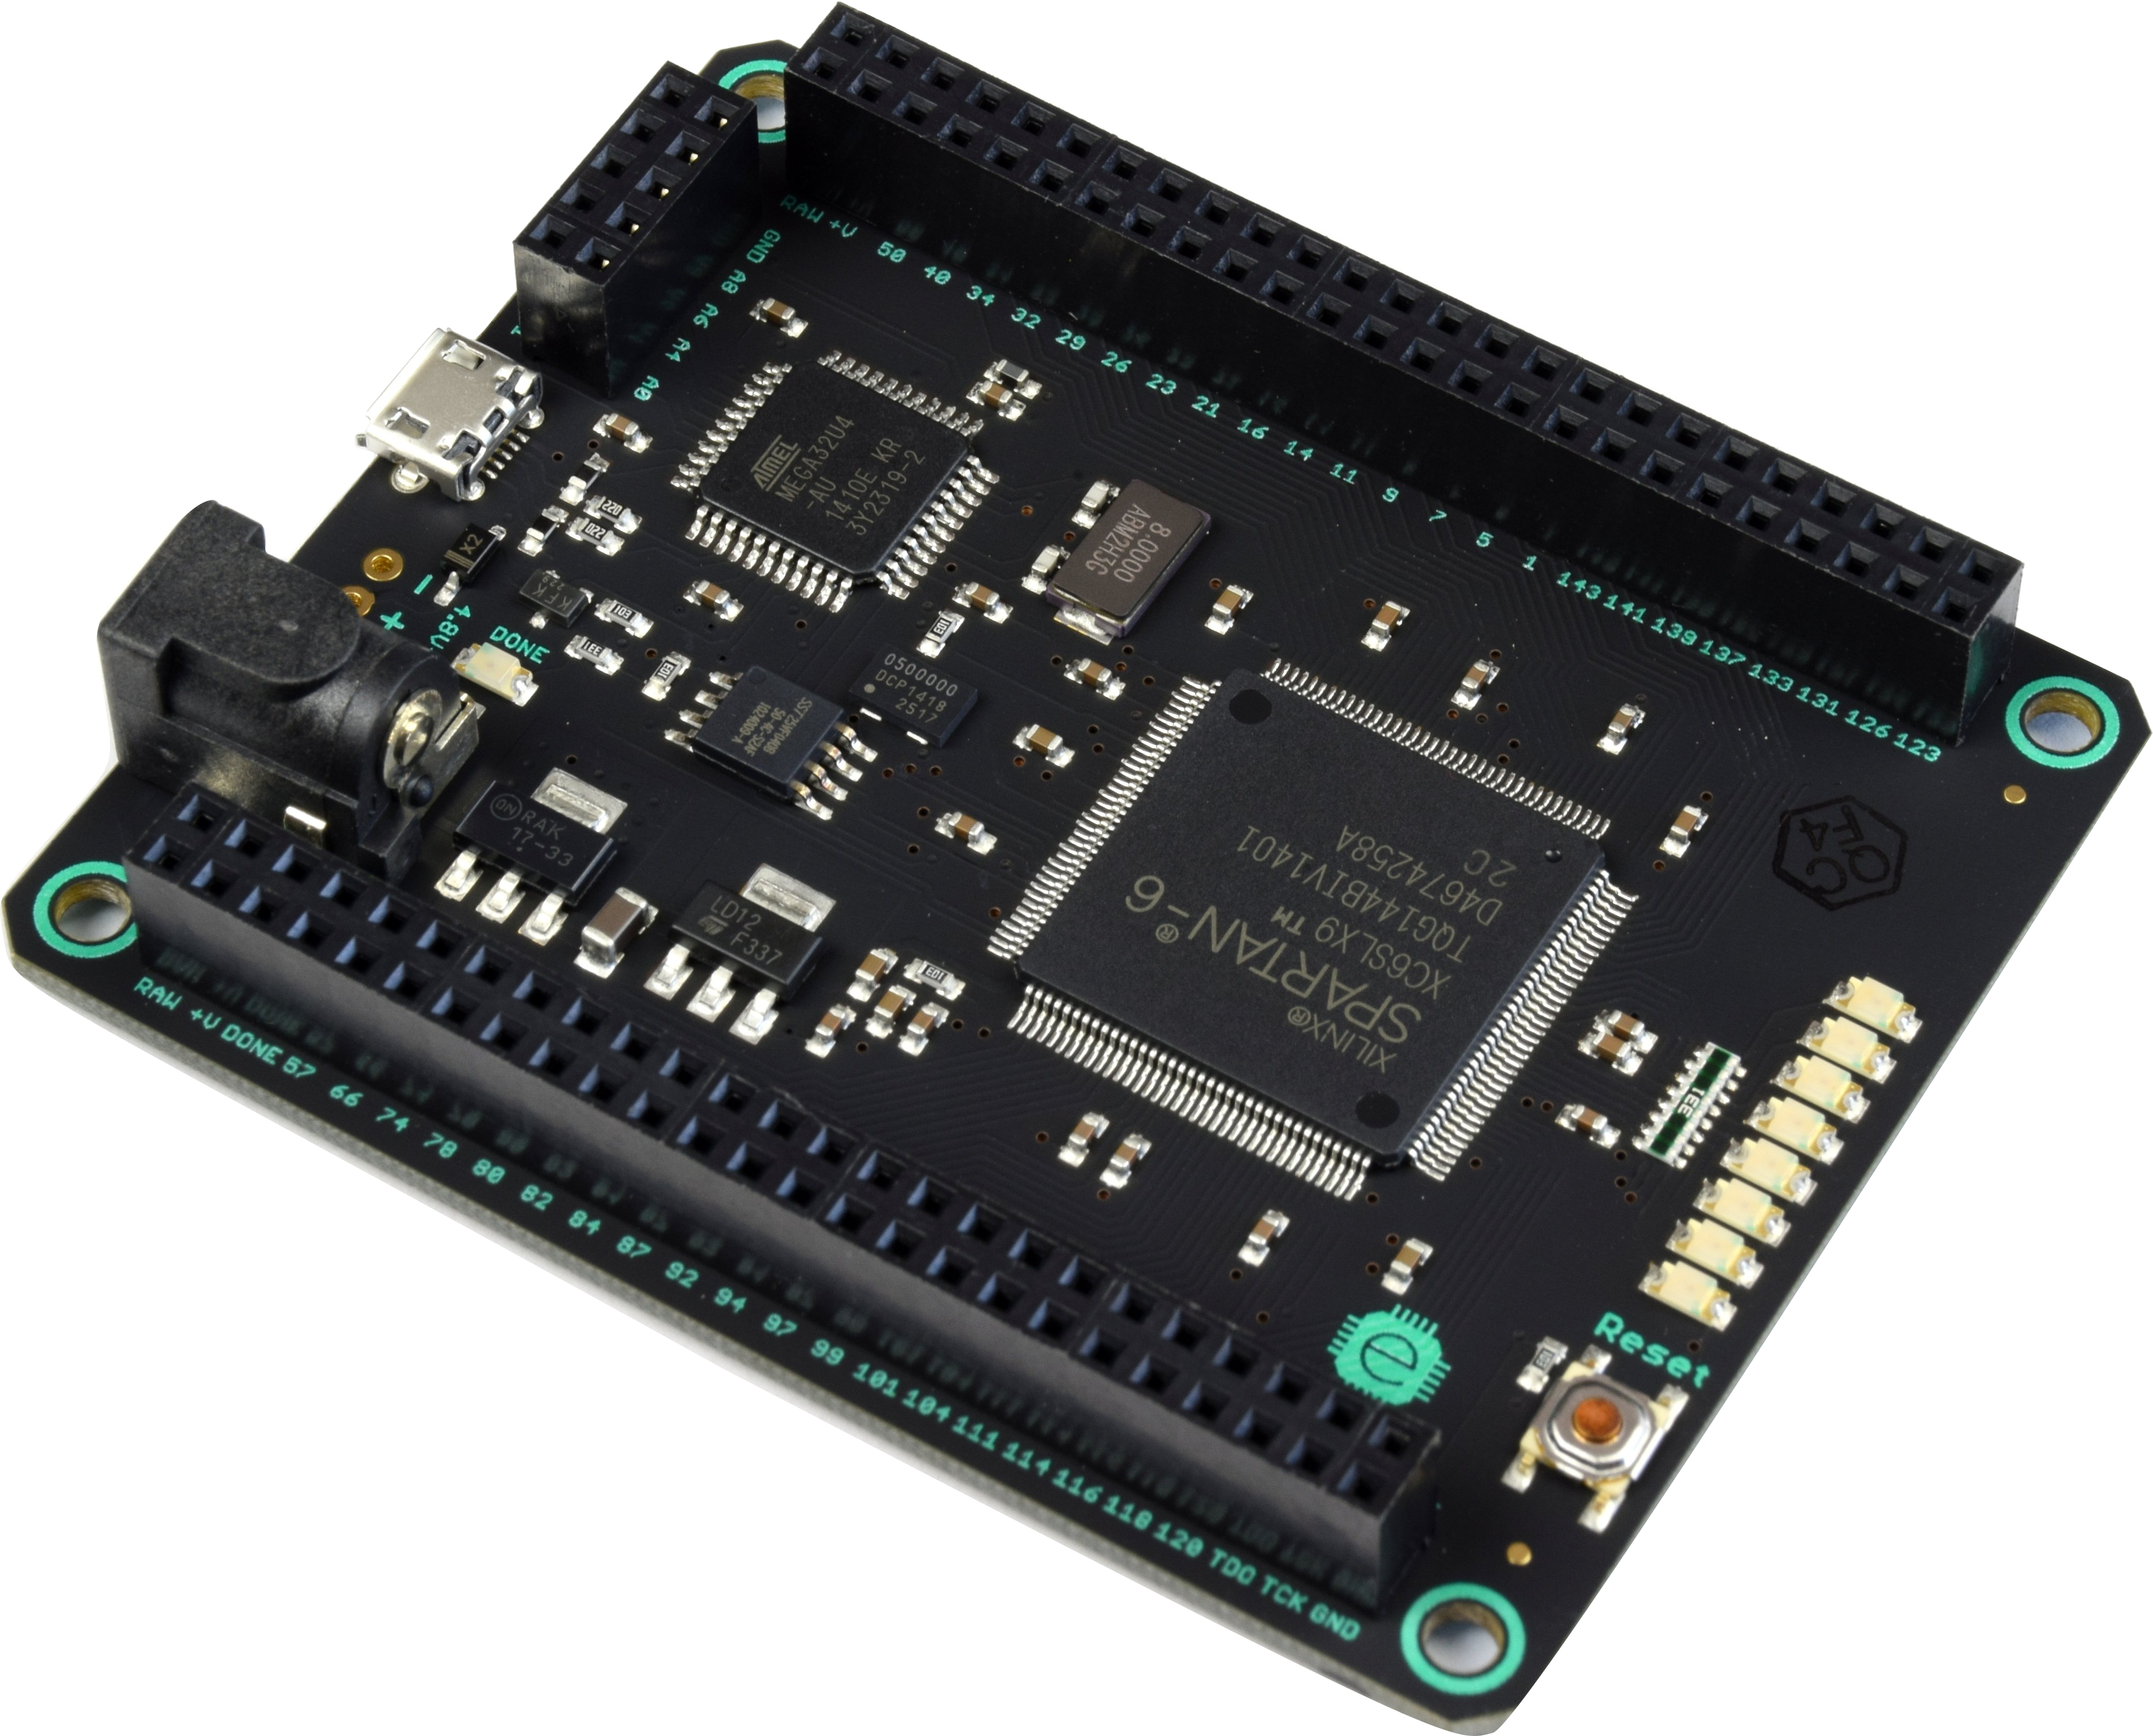
\includegraphics[width = 0.4\textwidth]{mojov3}
	\caption{Placa de prototipado rápido MOJO v3, diseñada por Embedded Micro}
	\label{mojo}
\end{figure}

La placa MOJO es una placa inspirada en el concepto de prototipado rápido. Para ello los puertos se disponen en un arreglo de pines a través de los cuales es posible acoplar cualquier dispositivo que uno necesite. Se dispone en el mercado otros circuitos, que los fabricantes denominan shields ({\it escudo} traducido al castellano), que encajan a la perfección en todos los pines y que contiene un set particular de perfiéricos útiles para propósito general. Estos shields, también, con el fin de satisfacer requerimientos especiales, pueden ser diseñados por uno mismo, o bien es posible adaptar con algunos cables las entradas a un dispositivo particular.\\

Además de estos shields, los diseñadores pensaron en que no sea necesario ninguna herramienta extra a la hora de programar la FPGA. Para ello, dotaron al sistema de un microcontrolador ATmega32U4 de Atmel y cargaron un programa bootloader, que se encarga de transferir la configuración del FPGA cargada desde una memoria flash incorporada al sistema con ese propósito particular, o trasmitida por el usuario desde una PC, a través de un transceptor USB que contiene el microcontrolador. Luego, este último es colocado en modo esclavo y se configura de forma tal que dota al sistema de una comunicación entre la FPGA y una PC, vía USB y se utiliza su ADC para leer los puertos analógicos.\\%Luego, entra en modo esclavo, lo que permite al usuario, a posterior poder usar para debug el sistema USB que posee el microcontrolador.\\

Una vez llegado a este punto, el lector podría preguntar con toda razón ¿por qué es necesario realizar un sistema de comunicación USB extra, si ya cuenta con un microcontrolador que se encarga de dicho asunto? La respuesta se basa en el ancho de banda del sistema de comunicación que dispone la placa. La línea de controladores ATmega incorpora puertos USB 2.0 full-speed. Esto quiere decir que puede enviar datos a una tasa de \SI{12}{\mega bp\second}. Además, la comunicación entre ambos chips se realiza via SPI (\(Serial Peripherical Interface\), o en español Interfaz Serie de Periféricos), comandada por un cristal de cuarzo de \SI{50}{\mega\hertz}, ofreciendo una velocidad de salida que puede resultar lenta a los fines de este trabajo. Se pretende dotar al sistema del mayor ancho de banda posible, utilizando la capacidad de USB 2.0 High-Speed, de hasta \SI{480}{\mega bp\second}.\\

